\chapter{Segmentación y Alineación automática}

Como la creación de recursos de manera manual es costosa, y los requerimientos de volúmen de información son altos, la generación automática o semi automática de recursos de habla toma gran relevancia en la investigación actual.

El procesamiento de grabaciones del dominio público para la creación de recursos para la investigación requiere la resolución de dos tareas concretas, que son la segmentación y la anotación definidas en el capítulo anterior.

\section{Segmentación basada en silencio}

Las segmentación basada en silencio es una respuesta natural al problema de como segmentar señales de voz, pues existe una correspondencia directa entre símbolos de puntuación y pausas en la voz. De igual manera en una señal de voz, los locutores requieren pausas para tomar aire, lo que permite que exista una cadencia en la señal y espacios donde realizar los cortes.

Para identificar el proceso de segmentación por silencios, es necesario entender cómo se almacenan las señales de voz digitalmente y cómo se puede procesar este tipo de datos.

La manera mas sencilla de representar digitalmente una señal de voz es haciendo el uso de la Modulación por Impulsos Codificados o PCM por sus siglas en inglés, donde por medio de un transductor análogo, se capturan las variaciones en la presión del aire y se registran como un rango de valores normalizado. El senso de la señal se hace periódicamente a una frecuencia determinada generando de esta manera una secuencia de valores que representa la señal. El proceso de representar la presión del aire en un segmento de tiempo se denomina cuantización, y para señales de audio se utilizan valores normalizados entre -127 y 128 representados por 8 bits a 16000 Hz de frecuencia.

En al figura \ref{img:pcm} se muestra la visualización de una grabación correspondiente a la palabra agua, extraída del corpus Open Speech Corpus de palabaras, en su longitud original y aumentada en un 500\% y 1000\% usando Audacity \cite{audacity}

\begin{figure}[H]
\caption{Representación visual de una señal de voz}
\label{img:pcm}
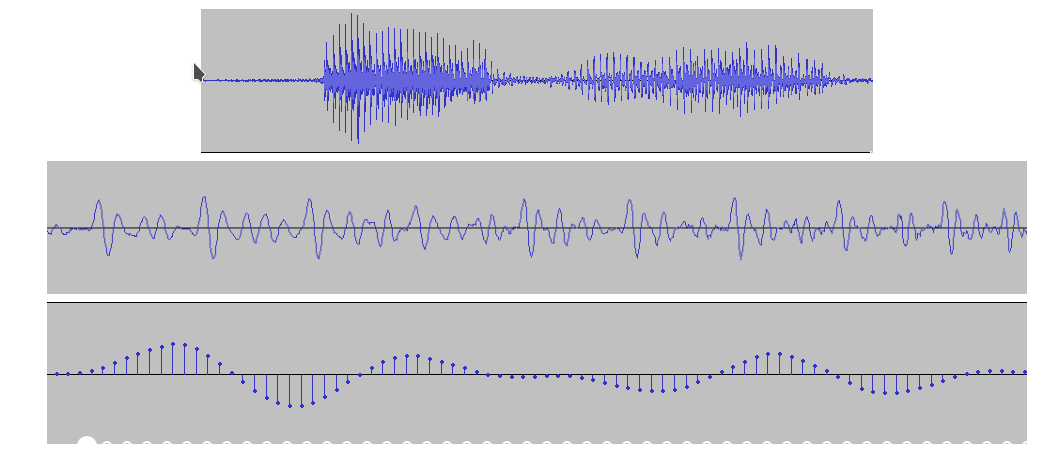
\includegraphics[width=\textwidth]{imagenes/04_01_pcm.png}
\end{figure}

Al hablar de silencio, nos referimos a ausencia total o parcial de sonido, lo cual se puede relacionar directamente con la intensidad de la señal en un segmento de tiempo.

Definiremos intensidad como la sumatoria de las energías en un periodo de tiempo  \cite{Jurafsky2000SpeechRecognition}    

\begin{equation}
\label{eq:energy}
I = \sum{x^2}  
\end{equation}

Esto nos daría un indicador de toda la señal, sin embargo, es útil realizar este análisis por pequeños segmentos del audio para identificar en conjunto cuales son los puntos donde la intensidad baja representa un espacio de silencio. Estos segmentos por lo general se definen en espacios de 25ms solapados cada 10ms \cite{Jurafsky2000SpeechRecognition}, lo cual da la idea de una señal continua, donde cada segmento comparte información con el anterior. 

Utilizando esta idea es posible tomar cualquier señal de voz, segmentarla cada 25ms y encontrar los segmentos consecutivos donde la intensidad sea baja o cercana a cero y estos segmentos consecutivos representarían pausas de silencio. Algunas consideraciones a tomar al usar esta aproximación es que incluso en medio de las señales de voz, existen subsegmentos donde la intensidad es baja, por ejemplo en la pronunciación de consonantes plosivas, como la b, c, d, g, p y t existe una interrupción momentánea y completa del flujo de aire, causando momentáneamente segmentos de silencio.

Con base en las anotaciones del corpus de experimentación fonética se determinó que la duración promedio de cada consonante plosiva es inferior a los 100ms. También, extrayendo información del corpus de pruebas se determinó que los espacios de silencio son de aproximadamente 500ms. Con esta información se decidió utilizar segmentos 250ms de longitud y desplazamiento de 100ms. Se determinan como silencios los conjuntos de cinco o más segmentos consecutivos de intensidad baja.

El criterio de silencio seleccionado como baja intensidad de múltiples segmentos consecutivos plantea retos con respecto al valor concreto de energía para determinar silencio o señal. Considerando que los locutores no grabaron a un volúmen estándar y que la relación ruido señal varía en todas las grabaciones es distinta, se propusieron dos aproximaciones para determinar los segmentos de silencio, la primera normalizando los valores de la señal y definiendo un umbral fijo de intensidad en proporción al valor mas alto de la grabación, considerando valores de 0.3, 0.15 y 0.15 que representan umbrales de intensidad del 30\%, 15\%, y 5\%. También se experimentó utilizando algoritmos de agrupamiento con dos centroides iniciales en 0 y la intensidad máxima. Los resultados se presentan en la tabla \ref{tab:resultados_segmentacion_silencios}.

\begin{table}[H]
\centering
\caption{Resultados de la segmentación por silencios}
% \caption{Speech English Corpus}
\label{tab:resultados_segmentacion_silencios}
\begin{tabular}{|l|l|}
\hline
\textbf{Umbral} & \textbf{Precisión}  \\ \hline
Fijo 30\%       & 57.01\%             \\  \hline
Fija 15\%       & 83.26\%             \\  \hline
Fija 5\%        & 69.05\%             \\  \hline
Dinámico        & 74.53\%             \\  \hline
\end{tabular}
\end{table}


\section{Alineación basada en duración de fonemas}

\textcolor{red}{WIP}

Utilizando la segmentación basada en silencios, para determinar cuales son los textos correspondientes se realiza una alineación basada en la duración estimada de un segmento de texto y la duración de los segmentos calculados. Para esto se tomó la anotación fonética para determinar la duración promedio y la desviación estándar de la duración de cada fonema. \macb{(La redacci\'on de este p\'arrafo se puede mejorar empezando por definir cu\'al es el siguiente objetivo y cu\'al es el input de dicho proceso. Ahora est\'a un poco confuso.)} Dicha información se puede ver en la tabla \ref{tab:duracion_promedio_fonemas} \macb{(Es importante aclarar cu\'al est\'andar se est\'a usando para los s\'imbolos de los fonemas. Tal vez en el cap\'itulo 3.)}

\begin{table}[H]
\centering
\caption{Distribución fonética}
\label{tab:duracion_promedio_fonemas}
\begin{tabular}{|l|l|l|}
\textbf{Fonema} &\multicolumn{1}{|p{2cm}|}{\textbf{Duración promedio}} & \multicolumn{1}{|p{2cm}|}{\textbf{Desviación estándar}} \\ \hline
sil & 0.6619 & 0.3700 \\ \hline
a   & 0.1421 & 0.0566 \\ \hline
o   & 0.1487 & 0.0607 \\ \hline
e   & 0.1204 & 0.0416 \\ \hline
n   & 0.1090 & 0.0442 \\ \hline
i   & 0.1294 & 0.0404 \\ \hline
l   & 0.1125 & 0.0530 \\ \hline
s   & 0.1811 & 0.1059 \\ \hline
t   & 0.0784 & 0.0507 \\ \hline
d   & 0.0877 & 0.0536 \\ \hline
R   & 0.0999 & 0.0517 \\ \hline
b   & 0.0826 & 0.0610 \\ \hline
r   & 0.0750 & 0.0254 \\ \hline
p   & 0.0692 & 0.0649 \\ \hline
j   & 0.1038 & 0.0659 \\ \hline
u   & 0.1441 & 0.0507 \\ \hline
m   & 0.1183 & 0.0515 \\ \hline
k   & 0.1224 & 0.0904 \\ \hline
g   & 0.1016 & 0.0970 \\ \hline
f   & 0.1402 & 0.0569  \\ \hline
c   & 0.1032 & 0.0838  \\ \hline
y   & 0.1118 & 0.0044  \\ \hline
C   & 0.1274 & 0.0248  \\ \hline
N   & 0.0575 & 0  \\ \hline
S   & 0.0927 & 0  \\ \hline
\end{tabular}
\end{table}

\section{Segmentación basada en información fonética de formantes en vocales}
\macb{informaci\'on fon\'etica podr\'ia ser ambiguo. Se podr\'ia usar el t\'ermino caracter\'isticas acusticas.}
\textcolor{red}{WIP}

La manera de entender los sonidos del lenguaje hablado ocurre por \macb{\st{por}} la similaridad de los sonidos emitidos por cualquier locutor. Estas maneras de articular cada fonema permite que todos ellos tengan la misma una composición acústica similar. \macb{Revisar este p\'arrafo. No es claro.}

Las vocales por ser sonidos de duración promedio mas alta y donde las características que las definen son pocas \macb{(Cu\'ales caracter\'isticas? Las vocales ocurren en el mismo espacio ac\'ustico que las consonantes.)}, únicamente la apertura de cuerdas bocales y la apertura de la boca, permiten que se caractericen utilizando una descomposición acústica. \macb{Revisar este p\'arrafo. Creo que aqu\'i estas hablando de la clasificaci\'on por manera de articulaci\'on. Para alguien que no est\'e familiarizado con el tema puede ser un poco confuso estos dos \'ultimos p\'arrafos. Se podr\'ia hacer una introducci\'on un poco m\'as clara sobre las posibles formas de clasificar los sonidos de un lenguaje, unidades contrastantes m\'inimas, fonemas.}

Al descomponer cualquier señal utilizando la transformada de Fourier \macb{(ver equaci\'on \ref{eq:fourier}), se obtienen se\~nales ra\'iz de cada onda compleja. Con las se\~nales de voz, los coeficientes m\'aximos  en el orden ascendente de la frecuencia se denominan formantes, y el formante 1 (f1) y el formante 2 (f2) representan efectivamente el fen\'omeno efectuado por las cuerda vocales vibrando y la resonancia dad por la cavidad bucal.} \macb{(Los formantes son harm\'onicos, la captura de estos se da en se\~nales de cualquier tipo, sea de voz u otro fen\'onmeno f\'isico, por ejemplo las se\~nales generadas por instrumentos musicales. Todos los formantes F1,F2,F3, etc. corresponden al pulso excitativo de la glotis y la resonancia en el tracto vocal)}

\macb{edit\'e la equaci\'on con los comandos que creo son los indicados, revisar si es as\'i lo que se quiere.}
\begin{equation}
\label{eq:fourier}    
f(x) = \frac{1}{2} \, a_{0} + \sum_{n=1}^{\infty} \left[
   a_{n}\,\mathbf{cos} (n\,x) + b_{n} \,\mathbf{sin} (n\,x) \right]
\end{equation}

\macb{\st{Se obtienen se\~nales ra\'iz de cada onda compleja. Con las se\~nales de voz, los coeficientes m\'aximos  en el orden ascendente de la frecuencia se denominan formantes, y el formante 1 (f1) y el formante 2 (f2) representan efectivamente el fen\'omeno efectuado por las cuerda vocales vibrando y la resonancia dad por la cavidad bucal.}}

\macb{\st{Para el idioma espa\~nol l}L}os formantes teóricos para \macb{las cinco vocales d}el español se muestra\macb{n} en la tabla \ref{tab:formantes_teoricos} \macb{tomada de [REF] %\cite{Bradlow1995}
. \st{, los cuales fueron tomados a partir locutores con dialecto peninsular y donde se muestra la distribuci\'on voc\'alica incluyendo los dos primeros formantes %\cite{Bradlow1995}
.} Dichos formantes fueron calculados promediando la medici\'on de formates F1 y F2 de varios locutores con dialecto peninsular.}

\begin{table}[H]
\centering
\caption{Formantes teóricos para vocales del español.}
\label{tab:formantes_teoricos}
\begin{tabular}{|l|l|l|l|l|}
\hline
\textbf{Vocal} & \textbf{f1} & \textbf{f2} & \textbf{std f1} & \textbf{std f2} \\ \hline
a   & 638 & 36 & 1353 & 84 \\ \hline
e   & 458 & 42 & 1800 & 131 \\ \hline
i   & 286 & 6  & 2200 & 131 \\ \hline
o   & 460 & 19 & 1019 & 99 \\ \hline
u   & 300 & 20 & 992  & 121 \\ \hline

\end{tabular}
\end{table}

También se realizó una observación de las vocales calculando sus formantes basados en la información extra\macb{\'i}da de las palabras anotadas fonéticamente. Esta información se encuentra en la tabla \ref{tab:formantes_observador} \macb{(Falta explicaci\'on de c\'omo se calcularon esos formantes, con PRAAT? con alguna librer\'ia de python?)}

\begin{table}[H]
\centering
\caption{Formantes teóricos para vocales del español}
\label{tab:formantes_observador}
\begin{tabular}{|l|l|l|l|l|}
\hline
\textbf{Vocal} & \textbf{f1} & \textbf{f2} & \textbf{std f1} & \textbf{std f2} \\ \hline
a   & 682.84 & 1347.66 & 73.77 & 93.04 \\ \hline
e   & 494.84 & 1619.97 & 55.49 & 132.84\\ \hline
i   & 382.33 & 1657.33 & 50.65 & 155.24 \\ \hline
o   & 506.24 & 1101.14 & 60.20 & 170.64\\ \hline
u   & 434.77 & 984.185 & 50.32 & 193.66\\ \hline

\end{tabular}
\end{table}

A partir de esta información se realizaron experimentos buscando la precisión en la identificación de las vocales\macb{\st{, tomando una}. Para ello se tom\'o la} distancia\macb{(te refieres a la norma L1?)} L1 de los dos primeros formantes \macb{\st{y},} aumentando un umbral definido fijo y \macb{\st{tambi\'en}} utilizando la desviación estándar sobre los formantes observados\macb{(Las enumeraciones se separan con comas o punto y comas. S\'olo hasta el final de la enumeraci\'on se usa la conjuci\'on `y')}. Adicionalmente a esto\macb{,}\macb{(Clausula introductoria va separada con coma.)} se entrenó un algoritmo de agrupación no supervizado\macb{,} K-means\macb{,} inicializando los centroides en los formantes observados \macb{en el corpus de prueba}. Los resultados se reportan en la tabla \ref{tab:resultados_vocales}

\macb{(Qu\'e quiere decir Te\'orica m\'as X? X Hz? kHz? Explicarlo en el caption de la tabla ayuda a entender mejor la informaci\'on de la tabla. Tambi\'en, poner negrita en el mejor resultado, esto ayuda al lector a identificar r\'apidamente qu\'e funcion\'o mejor. Esto \'ultimo tenerlo en cuenta en todas las tablas de resultados, o donde se quiera guiar la atenci\'on del lector.)}

\input{tablas/04_05_segmentación_vocalica}

Para entender los bajos resultados presentados por la aproximación basada en los formantes observados y su desviación\macb{(Indicar resultado o ubicaci\'on en la tabla. Por ejemplo, 55.73\% de precisi\'on,)}, \macb{se realiz\'o un an\'alisis visual.\st{s}S}e graficó \macb{simultaneamente la onda, los formantes F1 y F2 donde la intensidad superaba los 60 decibeles, es decir, $I > 60 dB$, y los formantes F1 y F2 promedio y sus desviaciones observados en el corpus. \st{sobre grabaciones con contenido de s\'olo las vocales, graficando los formantes 1 y 2 en espacios donde la intensidad superaba los 60 decibeles y graficando tambi\'en los formantes observados y su desviaci\'on est\'andar de las vocales a en la figura} Las figureas [REF 4.2-4.3] muestran un ejemplo de dicho an\'alisis. Los puntos indican los formantes calculados, en rojo F2 y en az\'ul F1. (Y explicar las lineas rojas, amarilla, verde. Recomiendo que los formantes observados sean graficados con la desviaci\'on st\'andar en transparencia. Tambi\'en, los dos formantes observados deber\'ian tener color distinto entre ellos y posiblemente en la misma escala de los calculados.)} 
%\ref{img:formantes_a} y e en la figura \ref{img:formantes_e}

% Ejemplo de cómo graficar la desviación estándar: https://i.stack.imgur.com/pDYIh.png


\macb{(Es mejor usar el nombre de los corpus para saber con certeza a cu\'al te refieres, o asignar un identificador en el cap\'itulo 3 que sea usado a trav\'es de todo el documento.)}

\begin{figure}[H]
\caption{Formantes de vocal A\macb{usar notaci\'on fon\'etica, por ejemplo /a/ en SAMPA, la letra A en SAMPA es una vocal del ingl\'es, igualmente con E.}}
\label{img:formantes_a}
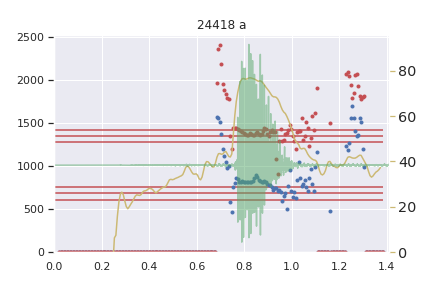
\includegraphics[width=\textwidth]{imagenes/04_02_a.png}
\end{figure}

\begin{figure}[H]
\caption{Formantes de vocal E}
\label{img:formantes_e}
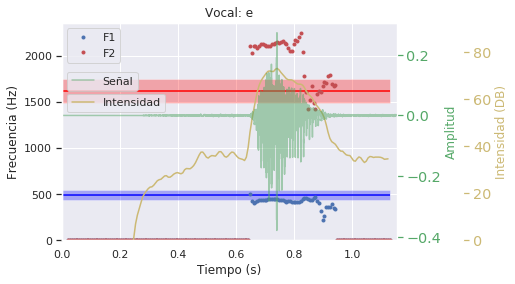
\includegraphics[width=\textwidth]{imagenes/04_02_e.png}
\end{figure}

% Esto debería estar arriba.
% En ambas figuras se muestra en verde la onda, en azul el formante 1 en rojo el formante dos, en amarillo la intensidad cuyo valor se encuentra en el eje derecho y en rojo y azul claro los rangos esperados siendo la línea centra el formante observado promedio y las lineas adyacentes los valores de sumar y restar la desviación estándar.

Como se observa en la grabación de la letra e \macb{C\'omo se observa esto? explicaci\'ion para alguien no familiarizado con se\~nales.}, hay un ambiente m\macb{\'a}s ruidoso, lo que hace que se capturen valores de formantes en lugares donde aún no hay señal de voz y aunque en los momentos donde la señal se estabiliza, los formantes tienden a acercarse a las bandas de frecuencia esperadas, esto no ocurre en todos los casos. \macb{Qu\'e quiere decir esta \'ultima frase?. Tambi\'en separar la oraci\'on en dos, ahora est\'a muy larga y dif\'icil de entender.}